% !Mode:: "TeX:UTF-8"
\chapter{相机与图像}
\label{cpt:5}
\begin{mdframed}  
	\textbf{主要目标}
	\begin{enumerate}[labelindent=0em,leftmargin=1.5em]
		\item 理解针孔相机的模型、内参与径向畸变参数。
		\item 理解一个空间点是如何投影到相机成像平面的。
		\item 掌握OpenCV的图像存储与表达方式。
		\item 学会基本的摄像头标定方法。
	\end{enumerate}
\end{mdframed} 

前面两讲中,我们介绍了“机器人如何表示自身位姿”的问题,部分地解释了SLAM经典模型中变量的含义和运动方程部分。本讲将讨论“机器人如何观测外部世界”,也就是观测方程部分。而在以相机为主的视觉SLAM中,观测主要是指\textbf{相机成像}的过程。

我们在现实生活中能看到大量的照片。在计算机中,一张照片由很多个像素组成,每个像素记录了色彩或亮度的信息。三维世界中的一个物体反射或发出的光线,穿过相机光心后,投影在相机的成像平面上。相机的感光器件接收到光线后,产生测量值,就得到了像素,形成了我们见到的照片。这个过程能否用数学原理来描述呢?本讲将首先讨论相机模型,说明投影关系具体如何描述,相机的内参是什么。同时,简单介绍双目成像与RGB-D相机的原理。然后,介绍二维照片像素的基本操作。最后,根据内外参数的含义,演示一个点云拼接的实验。
\newpage
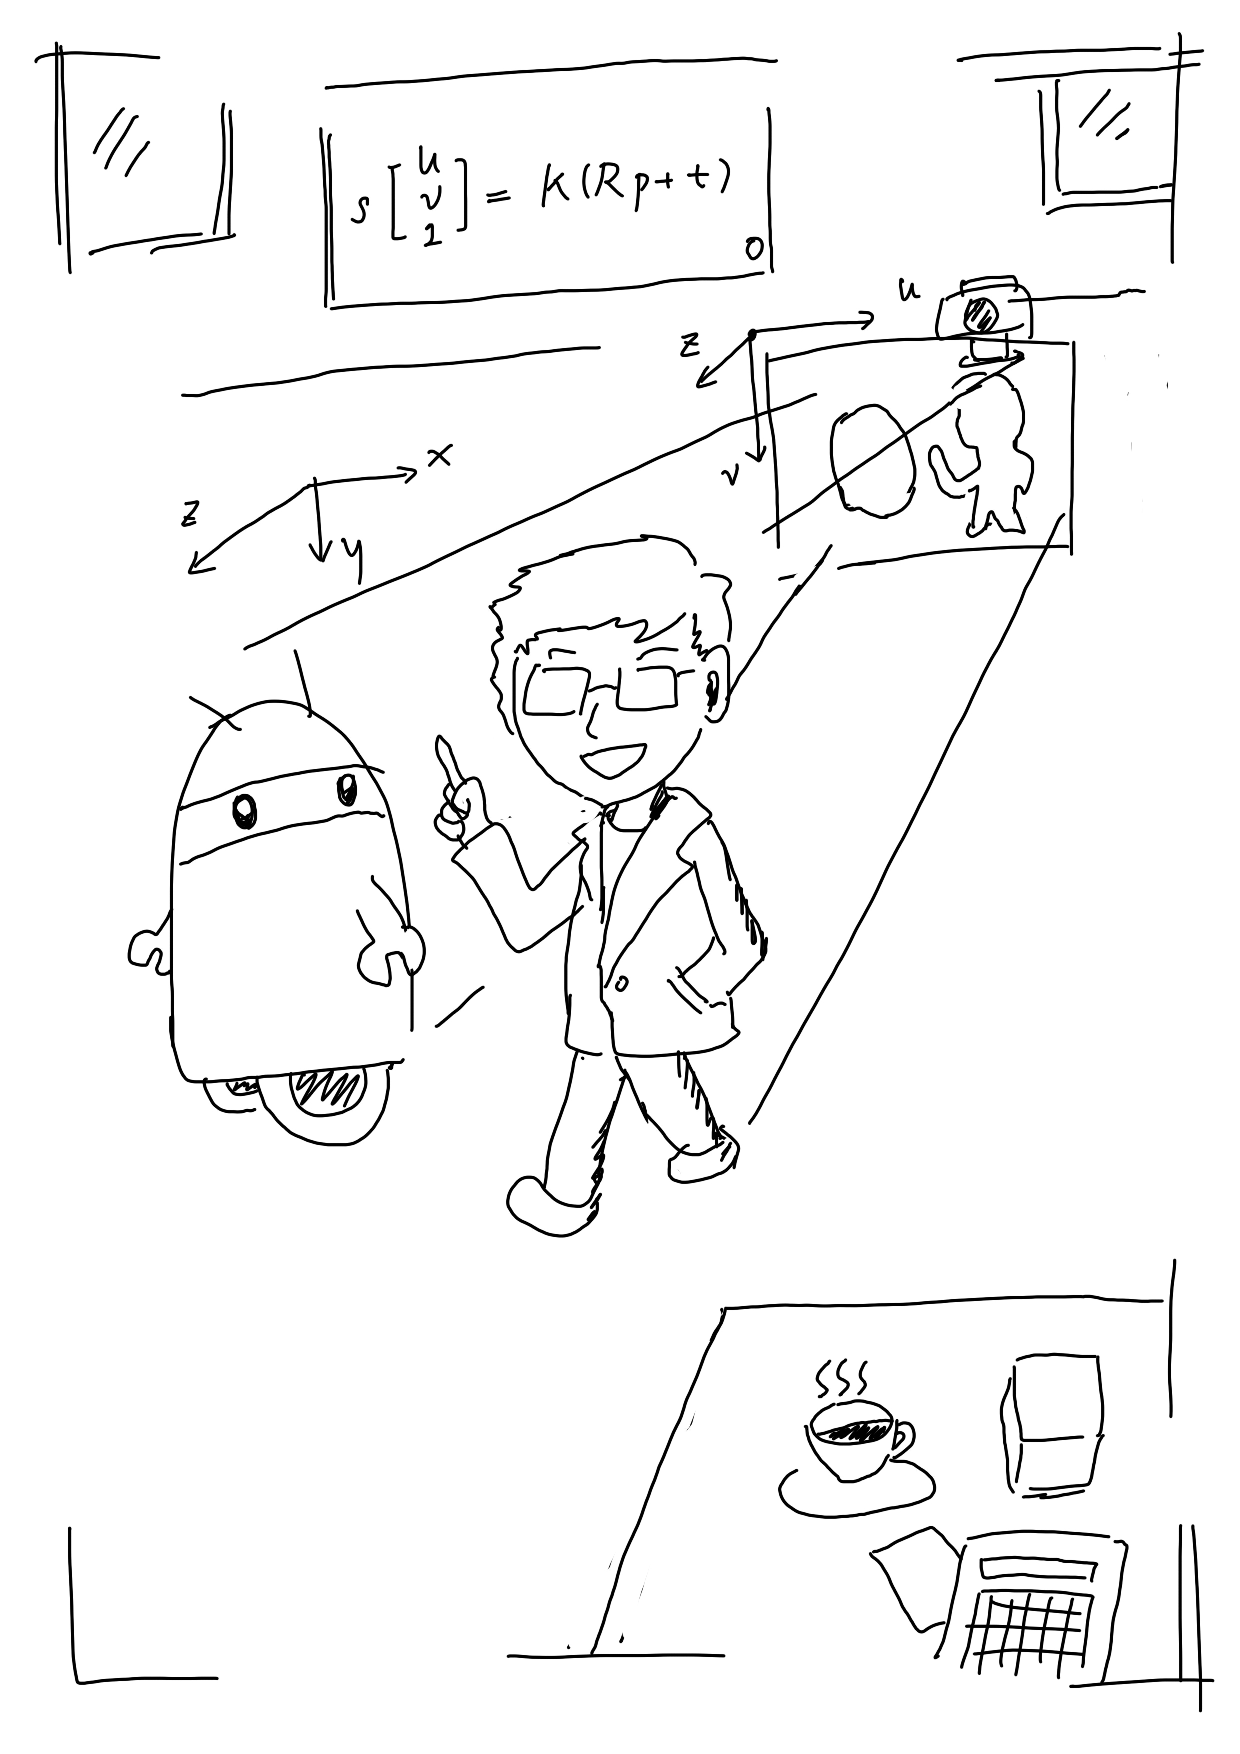
\includepdf{resources/other/ch5.pdf}

\newpage

% 此部分由贺一家编写
\section{相机模型}
相机将三维世界中的坐标点(单位为米)映射到二维图像平面(单位为像素)的过程能够用一个几何模型进行描述。这个模型有很多种,其中最简单的称为\textbf{针孔模型}。针孔模型是很常用而且有效的模型,它描述了一束光线通过针孔之后,在针孔背面投影成像的关系。在本书中我们用一个简单的针孔相机模型来对这种映射关系进行建模。同时,由于相机镜头上的透镜的存在,使得光线投影到成像平面的过程中会产生\textbf{畸变}。因此,我们使用针孔和畸变两个模型来描述整个投影过程。

在本节先给出相机的针孔模型,再对透镜的畸变模型进行讲解。这两个模型能够把外部的三维点投影到相机内部成像平面,构成相机的\textbf{内参数}(Intrinsics)。

\subsection{针孔相机模型}
在初中物理课堂上,我们可能都见过一个蜡烛投影实验:在一个暗箱的前方放着一支点燃的蜡烛,蜡烛的光透过暗箱上的一个小孔投影在暗箱的后方平面上,并在这个平面上形成一个倒立的蜡烛图像。在这个过程中,小孔模型能够把三维世界中的蜡烛投影到一个二维成像平面。同理,我们可以用这个简单的模型来解释相机的成像过程,如\autoref{fig:cameraModel}所示。

\begin{figure}[!ht]
	\centering
	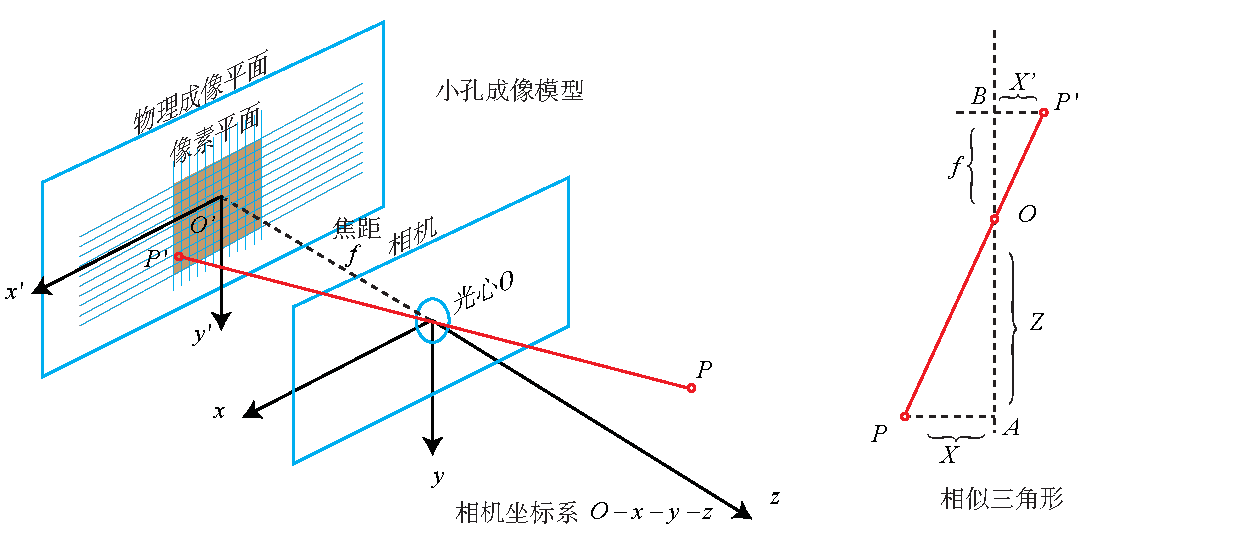
\includegraphics[width=.95\textwidth]{cameraModel/cameraModel.pdf}
	\caption{针孔相机模型。}
	\label{fig:cameraModel}
\end{figure}

现在来对这个简单的针孔模型进行几何建模。设$O-x-y-z$为相机坐标系,习惯上我们让$z$轴指向相机前方,$x$向右,$y$向下(此图我们应该站在左侧看右侧)。$O$为摄像机的\textbf{光心},也是针孔模型中的针孔。现实世界的空间点$P$,经过小孔$O$投影之后,落在物理成像平面$O'-x'-y'$上,成像点为$P'$。设$P$的坐标为$[X,Y,Z]^\mathrm{T}$,$P'$为$[X',Y',Z']^\mathrm{T}$,并且设物理成像平面到小孔的距离为$f$(焦距)。那么,根据三角形相似关系,有:
\clearpage
\begin{equation}
\frac{Z}{f} = -\frac{X}{{X'}} =-\frac{Y}{{Y'}}.
\end{equation}
其中负号表示成的像是倒立的。不过,实际相机得到的图像并不是倒像(否则相机的使用会非常不方便)。为了让模型更符合实际,我们可以等价地把成像平面对称地放到相机前方,和三维空间点一起放在摄像机坐标系的同一侧,如\autoref{fig:planes}所示。这样做可以把公式中的负号去掉,使式子更加简洁:

\begin{equation}
\frac{Z}{f} = \frac{X}{{X'}} =\frac{Y}{{Y'}}.
\end{equation}

\begin{figure}[!htp]
	\centering
	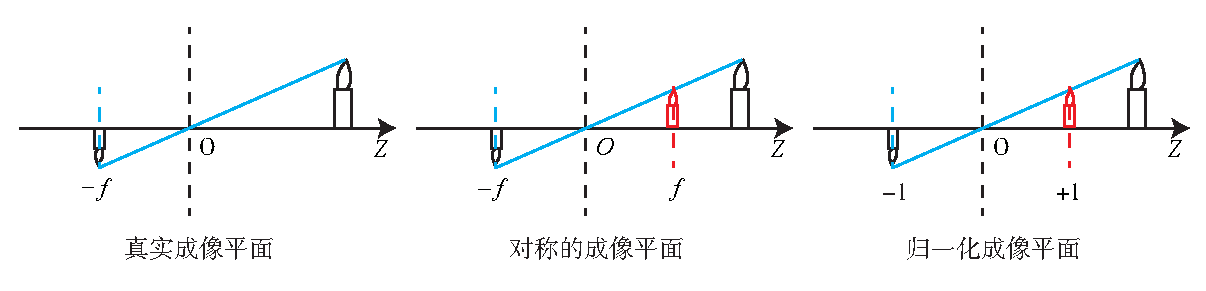
\includegraphics[width=1.0\textwidth]{cameraModel/planes.pdf}
	\caption{真实成像平面,对称成像平面,归一化成像平面的图示。}
	\label{fig:planes}
\end{figure}

把$X', Y'$放到等式左侧,整理得:

\begin{equation}\label{eq:P2Pprime}
\begin{array}{l}
X' = f\frac{X}{Z}\\
Y' = f\frac{Y}{Z}
\end{array}.
\end{equation}

读者可能要问,为什么我们可以看似随意地把成像平面挪到前方呢?这只是我们处理真实世界与相机投影的数学手段,并且,大多数相机输出的图像并不是倒像——相机自身的软件会帮你翻转这张图像,所以我们实际得到的是正像,也就是对称的成像平面上的像。所以,尽管从物理原理来说,小孔成像应该是倒像,但由于我们对图像作了预处理,所以理解成在对称平面上的像并不会带来什么坏处。于是,在不引起歧义的情况下,我们也不加限制地称后一种情况为针孔模型。

式\eqref{eq:P2Pprime}描述了点$P$和它的像之间的空间关系,这里所有点的单位都可理解成米,比如焦距是0.2米,$X'$是0.14米。不过,在相机中,我们最终获得的是一个个的像素,这还需要在成像平面上对像进行采样和量化。为了描述传感器将感受到的光线转换成图像像素的过程,我们设在物理成像平面上固定着一个像素平面$o-u-v$。我们在像素平面得到了$P'$的\textbf{像素坐标}:$[u,v]^\mathrm{T}$。

\textbf{像素坐标系}\footnote{或图像坐标系,见本讲第2节。}通常的定义方式是:原点$o'$位于图像的左上角,$u$轴向右与$x$轴平行,$v$轴向下与$y$轴平行。像素坐标系与成像平面之间,相差了一个\textbf{缩放}和一个\textbf{原点的平移}。我们设像素坐标在$u$轴上缩放了$\alpha$倍,在$v$上缩放了$\beta$倍。同时,原点平移了$[c_x, c_y]^\mathrm{T}$。那么,$P'$的坐标与像素坐标$[u,v]^\mathrm{T}$的关系为:

\begin{equation}
\label{eq:project2pixel1} 
\left\{
\begin{matrix} 
u=\alpha X' + c_x\\ 
v=\beta Y' + c_y
\end{matrix}
\right. .
\end{equation}

代入式\eqref{eq:P2Pprime}并把$\alpha f$合并成$f_x$,把$\beta f$合并成$f_y$,得:
\begin{equation}
\left\{
\begin{matrix} 
u=f_x\frac{X}{Z} + c_x\\ 
v=f_y\frac{Y}{Z} + c_y
\end{matrix}
\right. .
\end{equation}

其中,$f$的单位为米,$\alpha,\beta$的单位为像素/米,所以$f_x,f_y$和$c_x, c_y$的单位为像素。把该式写成矩阵形式会更加简洁,不过左侧需要用到齐次坐标,右侧则是非齐次坐标:

\begin{equation}
\label{eq:intrinmatrix} 
\begin{pmatrix} u\\ v\\ 1 \end{pmatrix}=\frac{1}{Z}\begin{pmatrix} f_x & 0&c_x \\ 0& f_y& c_y\\ 0&0 & 1 \end{pmatrix}\begin{pmatrix} X\\ Y\\ Z \end{pmatrix} 
\buildrel \Delta \over =\frac{1}{Z} \bm{K} \bm{P}.
\end{equation}

我们按照传统的习惯把$Z$挪到左侧:
\begin{equation}
Z \begin{pmatrix} u\\ v\\ 1 \end{pmatrix}= \begin{pmatrix} f_x & 0&c_x \\ 0& f_y& c_y\\ 0&0 & 1 \end{pmatrix}\begin{pmatrix} X\\ Y\\ Z \end{pmatrix} 
\buildrel \Delta \over = \bm{K} \bm{P}.
\end{equation}
该式中,我们把中间的量组成的矩阵称为相机的\textbf{内参数矩阵}(Camera Intrinsics)$\bm{K}$。通常认为,相机的内参在出厂之后是固定的,不会在使用过程中发生变化。有的相机生产厂商会告诉你相机的内参,而有时需要你自己确定相机的内参,也就是所谓的\textbf{标定}。鉴于标定算法业已成熟(如著名的单目棋盘格张正友标定法\textsuperscript{\cite{Zhang1999}}),这里就不介绍了。

有内参,自然也有相对的外参。在式~\eqref{eq:intrinmatrix}~中,我们使用的是$P$在相机坐标系下的坐标,但实际上由于相机在运动,所以$P$的相机坐标应该是它的世界坐标(记为$\bm{P}_w$)根据相机的当前位姿变换到相机坐标系下的结果。相机的位姿由它的旋转矩阵$\bm{R}$和平移向量$\bm{t}$来描述。那么有:

\begin{equation}
\label{eq:cameraprojection}
Z \bm{P}_{uv}=
Z \left[ \begin{array}{l}
u\\
v\\
1
\end{array} \right] = \bm{K} \left( {\bm{R}{ \bm{P}_w} + \bm{t}} \right) =  \bm{K} \bm{T} \bm{P}_w .
\end{equation}
注意后一个式子隐含了一次齐次坐标到非齐次坐标的转换(你能看出来吗?)\footnote{即,在$\bm{T}\bm{P}$中使用齐次坐标,再转化为非齐次坐标,再与$\bm{K}$相乘。}。它描述了$P$的世界坐标到像素坐标的投影关系。其中,相机的位姿$\bm{R},\bm{t}$又称为相机的\textbf{外参数}(Camera Extrinsics)\footnote{在机器人或自动驾驶车辆中,外参有时也解释成相机坐标系到机器人本体坐标系之间的变换,描述“相机安装在什么地方”。}。相比于不变的内参,外参会随着相机运动发生改变,同时也是SLAM中待估计的目标,代表着机器人的轨迹。
%
%上式两侧都是齐次坐标。因为齐次坐标乘上非零常数后表达同样的含义,所以可以简单地把$Z$去掉:
%\begin{equation}
%\bm{P}_{uv}=\bm{K} \bm{T} \bm{P}_w .
%\end{equation}
%但这样等号意义就变了,成为在齐次坐标下相等的概念,相差了一个非零常数。为了避免麻烦,我们还是从传统意义上来定义书写等号。
%这里还是提一下隐含着的齐次到非齐次的变换。

投影过程还可以从另一个角度来看。式\eqref{eq:cameraprojection}表明,我们可以把一个世界坐标点先转换到相机坐标系,再除掉它最后一维的数值(即该点距离相机成像平面的深度),这相当于把最后一维进行\textbf{归一化处理},得到点$P$在相机\textbf{归一化平面}上的投影:
\begin{equation}
\left( {\bm{R}{\bm{P}_w} + \bm{t}} \right) = \underbrace{\left[ X,Y,Z\right]^\mathrm{T}}_{\text{相机坐标}} \to \underbrace {\left[ {X/Z,Y/Z,1} \right]^\mathrm{T}}_{\text{归一化坐标}}.
\end{equation}
\textbf{归一化坐标}可看成相机前方\footnote{注意在实际计算中需要检查$Z$是否为正,因为负数$Z$也可以通过这个方式得到归一化平面上的一个点,但相机并不会拍到成像平面后方的景物。}$z=1$处的平面上的一个点,这个$z=1$平面也称为\textbf{归一化平面}。归一化坐标再左乘内参就得到了像素坐标,所以我们可以把像素坐标$[u,v]^\mathrm{T}$看成对归一化平面上的点进行量化测量的结果。从这个模型中也可以看出,如果对相机坐标同时乘以任意非零常数,归一化坐标都是一样的,这说明\textbf{点的深度在投影过程中被丢失了},所以单目视觉中没法得到像素点的深度值。

\subsection{畸变}
为了获得好的成像效果,我们在相机的前方加了透镜。透镜的加入对成像过程中光线的传播会产生新的影响:一是透镜自身的形状对光线传播的影响,二是在机械组装过程中,透镜和成像平面不可能完全平行,这也会使得光线穿过透镜投影到成像面时的位置发生变化。

由透镜形状引起的\textbf{畸变}(Distortion,也叫失真)称为\textbf{径向畸变}。在针孔模型中,一条直线投影到像素平面上还是一条直线。可是,在实际拍摄的照片中,摄像机的透镜往往使得真实环境中的一条直线在图片中变成了曲线\footnote{是的,它不再直了,而是变成弯的。如果往里弯,称为桶形失真;往外弯则是枕形失真。}。越靠近图像的边缘,这种现象越明显。由于实际加工制作的透镜往往是中心对称的,这使得不规则的畸变通常径向对称。它们主要分为两大类:\textbf{桶形畸变}和\textbf{枕形畸变},如\autoref{fig:distortion}所示。
\begin{figure}[!t]
    \centering
    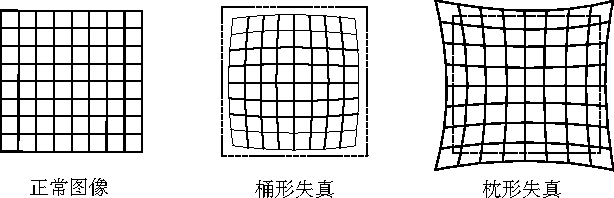
\includegraphics[width=0.7\textwidth]{cameraModel/distortion.pdf}
    \caption{径向畸变的两种类型。}
    \label{fig:distortion}
\end{figure}

桶形畸变是由于图像放大率随着与光轴之间的距离增加而减小,而枕形畸变则恰好相反。在这两种畸变中,穿过图像中心和光轴有交点的直线还能保持形状不变。

除了透镜的形状会引入径向畸变外,在相机的组装过程中由于不能使透镜和成像面严格平行也会引入\textbf{切向畸变},如\autoref{fig:tangen}所示。
\begin{figure}[!t]
    \centering
    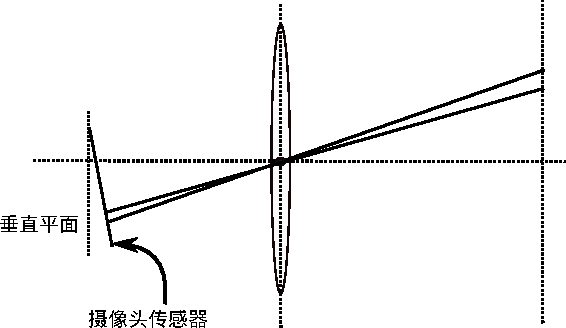
\includegraphics[width=0.7\textwidth]{cameraModel/tangen.pdf}
    \caption{切向畸变来源示意图。}
    \label{fig:tangen}
\end{figure}

为更好地理解径向畸变和切向畸变,我们用更严格的数学形式对两者进行描述。考虑\textbf{归一化平面}上的任意一点$\bm{p}$,它的坐标为$[x,y]^\mathrm{T}$,也可写成极坐标的形式$[r,\theta]^\mathrm{T}$,其中$r$表示点$\bm{p}$与坐标系原点之间的距离,$\theta$表示与水平轴的夹角。径向畸变可看成坐标点沿着长度方向发生了变化,也就是其距离原点的长度发生了变化。切向畸变可以看成坐标点沿着切线方向发生了变化,也就是水平夹角发生了变化。通常假设这些畸变呈多项式关系,即:
\begin{equation}
\label{eq:distortion} 
\begin{matrix}
x_\mathrm{distorted} = x(1+k_1r^2+k_2r^4+k_3r^6)\\
y_\mathrm{distorted} = y(1+k_1r^2+k_2r^4+k_3r^6)
\end{matrix}.
\end{equation}
其中$[x_\mathrm{distorted},y_\mathrm{distorted}]^\mathrm{T}$是畸变后点的\textbf{归一化坐标}。另一方面,对于\textbf{切向畸变},可以使用另外的两个参数$p_1,p_2$来进行纠正:
\begin{equation}
\label{eq:tangen} 
\begin{matrix}
x_\mathrm{distorted} = x+2p_1xy+p_2(r^2+2x^2)\\
y_\mathrm{distorted} = y+p_1(r^2+2y^2)+2p_2xy
\end{matrix}. 
\end{equation}

因此,联合式\eqref{eq:distortion}和式\eqref{eq:tangen},对于相机坐标系中的一点$\bm{P}$,我们能够通过5个畸变系数找到这个点在像素平面上的正确位置:

\begin{enumerate}
\item 将三维空间点投影到归一化图像平面。设它的归一化坐标为$[x,y]^\mathrm{T}$。

\item 对归一化平面上的点计算径向畸变和切向畸变。
\begin{equation}
\left\{\begin{matrix} x_\mathrm{distorted} =x(1+k_1r^2+k_2r^4+k_3r^6)+2p_1xy+p_2(r^2+2x^2)\\ 
y_\mathrm{distorted} = y(1+k_1r^2+k_2r^4+k_3r^6)+p_1(r^2+2y^2)+2p_2xy
\end{matrix}\right. .
\end{equation}
\item 将畸变后的点通过内参数矩阵投影到像素平面,得到该点在图像上的正确位置。
\begin{equation}
\left\{\begin{matrix} u=f_x x_\mathrm{distorted} + c_x\\ v=f_y y_\mathrm{distorted} + c_y\end{matrix}\right. .
\end{equation}
\end{enumerate}

在上面的纠正畸变的过程中,我们使用了5个畸变项。实际应用中,可以灵活选择纠正模型,比如只选择$k_1,p_1,p_2$这3项等。

在这一节中,我们对相机的成像过程使用针孔模型进行了建模,也对透镜引起的径向畸变和切向畸变进行了描述。实际的图像系统中,学者们提出了很多其他的模型,比如相机的仿射模型和透视模型等,同时也存在很多其他类型的畸变。考虑到视觉SLAM中一般都使用普通的摄像头,针孔模型及径向畸变和切向畸变模型已经足够,因此,我们不再对其他模型进行描述。

值得一提的是,存在两种去畸变处理(Undistort,或称畸变校正)做法。我们可以选择先对整张图像进行去畸变,得到去畸变后的图像,然后讨论此图像上的点的空间位置。或者,也可以从畸变图像上的某个点出发,按照畸变方程,讨论其畸变前的空间位置。二者都是可行的,不过前者在视觉SLAM中似乎更加常见一些。所以,当一个图像去畸变之后,我们就可以直接用针孔模型建立投影关系,而不用考虑畸变了。因此,在后文的讨论中,我们可以直接假设图像已经进行了去畸变处理。

最后,我们小结一下单目相机的成像过程:

\begin{enumerate}
	\item 首先,世界坐标系下有一个固定的点$P$,世界坐标为$\bm{P}_w$。
	\item 由于相机在运动,它的运动由$\bm{R}, \bm{t}$或变换矩阵$\bm{T} \in \mathrm{SE}(3)$描述。$P$的相机坐标为$\bm{\tilde{P}}_c = \bm{R} \bm{P}_w + \bm{t}$。
	\item 这时的$\bm{\tilde{P}}_c$的分量为$X,Y,Z$,把它们投影到归一化平面$Z=1$上,得到$P$的归一化坐标:$\bm{P}_c = [X/Z, Y/Z, 1]^\mathrm{T}$\footnote{注意到$Z$可能小于1,说明该点位于归一化平面后面,它可能不会在相机平面上成像,实践当中要检查一次。}。
	\item 有畸变时,根据畸变参数计算$\bm{P}_c$发生畸变后的坐标。
	\item 最后,$P$的归一化坐标经过内参后,对应到它的像素坐标:$\bm{P}_{uv} = \bm{K} \bm{P}_c$。
\end{enumerate}

综上所述,我们一共谈到了四种坐标:世界坐标、相机坐标、归一化坐标和像素坐标。请读者厘清它们的关系,它反映了整个成像的过程。

\subsection{双目相机模型}
针孔相机模型描述了单个相机的成像模型。然而,仅根据一个像素,我们无法确定这个空间点的具体位置。这是因为,从相机光心到归一化平面连线上的所有点,都可以投影至该像素上。只有当$P$的深度确定时(比如通过双目或RGB-D相机),我们才能确切地知道它的空间位置。如\autoref{fig:pixelLocation}~所示。

\begin{figure}[!ht]
	\centering
	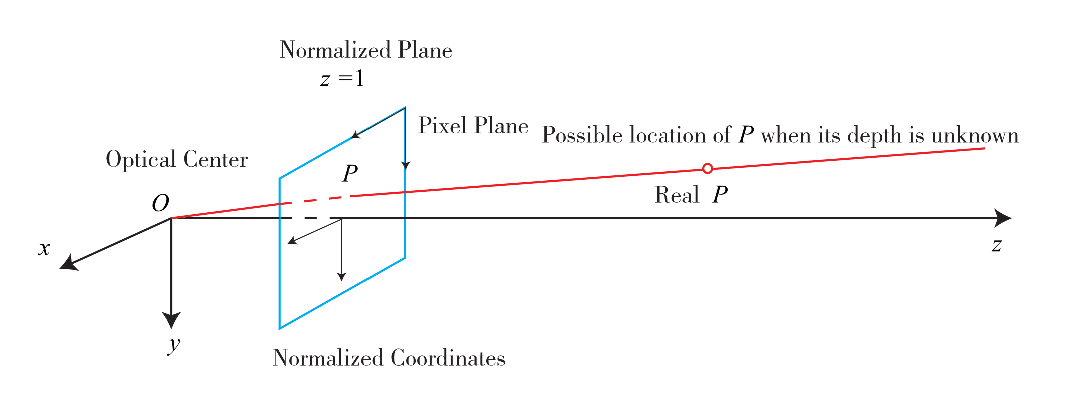
\includegraphics[width=1.0\textwidth]{cameraModel/pixelLocation.pdf}
	\caption{像素点可能存在的位置。}
	\label{fig:pixelLocation}
\end{figure}

测量像素距离(或深度)的方式有很多种,比如人眼就可以根据左右眼看到的景物差异(或称视差)来判断物体离我们的距离。双目相机的原理亦是如此:通过同步采集左右相机的图像,计算图像间视差,来估计每一个像素的深度。下面简单讲讲双目相机的成像原理(如\autoref{fig:stereoCamera}~所示)。

双目相机一般由左眼相机和右眼相机两个水平放置的相机组成。当然也可以做成上下两个目\footnote{那样的话外观会有些奇特。},不过我们见到的主流双目都是做成左右形式的。在左右双目相机中,我们可以把两个相机都看作针孔相机。它们是水平放置的,意味着两个相机的光圈中心都位于$x$轴上。两者之间的距离称为双目相机的\textbf{基线}(Baseline,记作$b$),是双目相机的重要参数。

\begin{figure}[!ht]
	\centering
	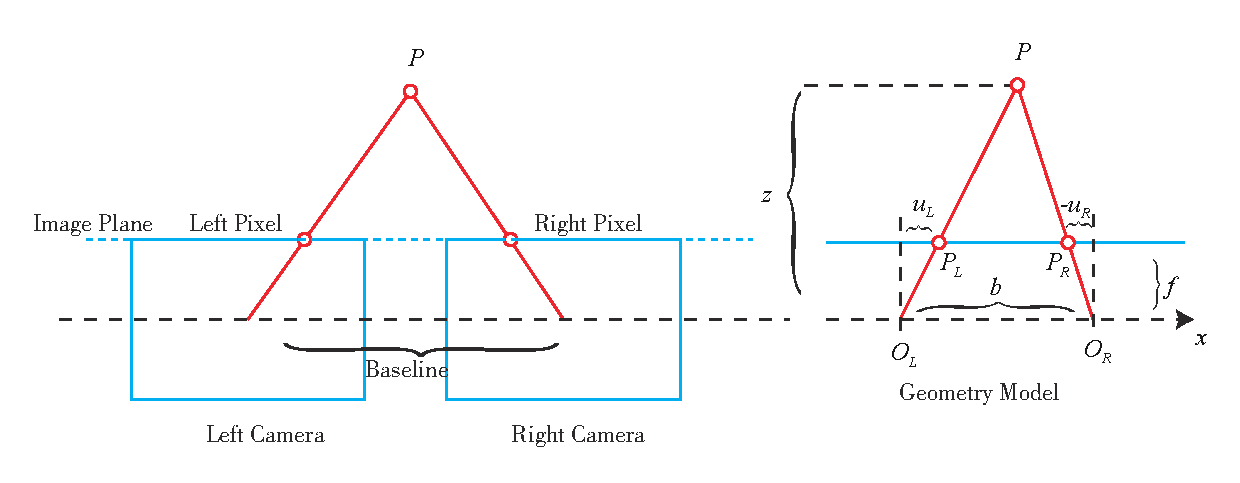
\includegraphics[width=1.0\textwidth]{cameraModel/stereoCamera.pdf}
	\caption{双目相机的成像模型。$O_L,O_R$为左右光圈中心,方框为成像平面,$f$为焦距。$u_L$和$u_R$为成像平面的坐标。请注意,按照图中坐标定义,$u_R$应该是负数,所以图中标出的距离为$-u_R$。}
	\label{fig:stereoCamera}
\end{figure}

现在,考虑一个空间点$P$,它在左眼相机和右眼相机各成一像,记作$P_L, P_R$。由于相机基线的存在,这两个成像位置是不同的。理想情况下,由于左右相机只在$x$轴上有位移,因此$P$的像也只在$x$轴(对应图像的$u$轴)上有差异。记它的左侧坐标为$u_L$,右侧坐标为$u_R$,几何关系如\autoref{fig:stereoCamera}右侧所示。根据$\triangle PP_LP_R$和$\triangle PO_LO_R$的相似关系,有:

\begin{equation}
\frac{{z - f}}{z} = \frac{{b - {u_L} + {u_R}}}{b}.
\end{equation}

稍加整理,得:
\begin{equation}
z = \frac{{fb}}{d}, \quad d \buildrel \Delta \over = {u_L} - {u_R}.
\end{equation}
其中$d$定义为左右图的横坐标之差,称为\textbf{视差}(Disparity)。根据视差,我们可以估计一个像素与相机之间的距离。视差与距离成反比:视差越大,距离越近\footnote{读者可以自己用眼睛模拟一下。}。同时,由于视差最小为一个像素,于是双目的深度存在一个理论上的最大值,由$fb$确定。我们看到,当基线越长时,双目能测到的最大距离就会越远;反之,小型双目器件则只能测量很近的距离。类比地,我们人眼在看非常远的物体时(如很远的飞机),通常不能准确判断它的距离。

虽然由视差计算深度的公式很简洁,但视差$d$本身的计算却比较困难。我们需要确切地知道左眼图像某个像素出现在右眼图像的哪一个位置(即对应关系),这件事亦属于“人类觉得容易而计算机觉得困难”的任务。当我们想计算每个像素的深度时,其计算量与精度都将成为问题,而且只有在图像纹理变化丰富的地方才能计算视差。由于计算量的原因,双目深度估计仍需要使用GPU或FPGA来实时计算。这将在第13讲中提到。

\subsection{RGB-D相机模型}
相比于双目相机通过视差计算深度的方式,RGB-D相机的做法更为“主动”一些,它能够主动测量每个像素的深度。目前的RGB-D相机按原理可分为两大类(见\autoref{fig:RGBDCamera}~):

\begin{enumerate}
	\item 通过\textbf{红外结构光}(Structured Light)来测量像素距离的。例子有Kinect 1代、Project Tango 1 代、Intel RealSense等。
	\item 通过\textbf{飞行时间法}(Time-of-flight,ToF)原理测量像素距离的。例子有Kinect 2代和一些现有的ToF传感器等。
\end{enumerate}

\begin{figure}[!ht]
	\centering
	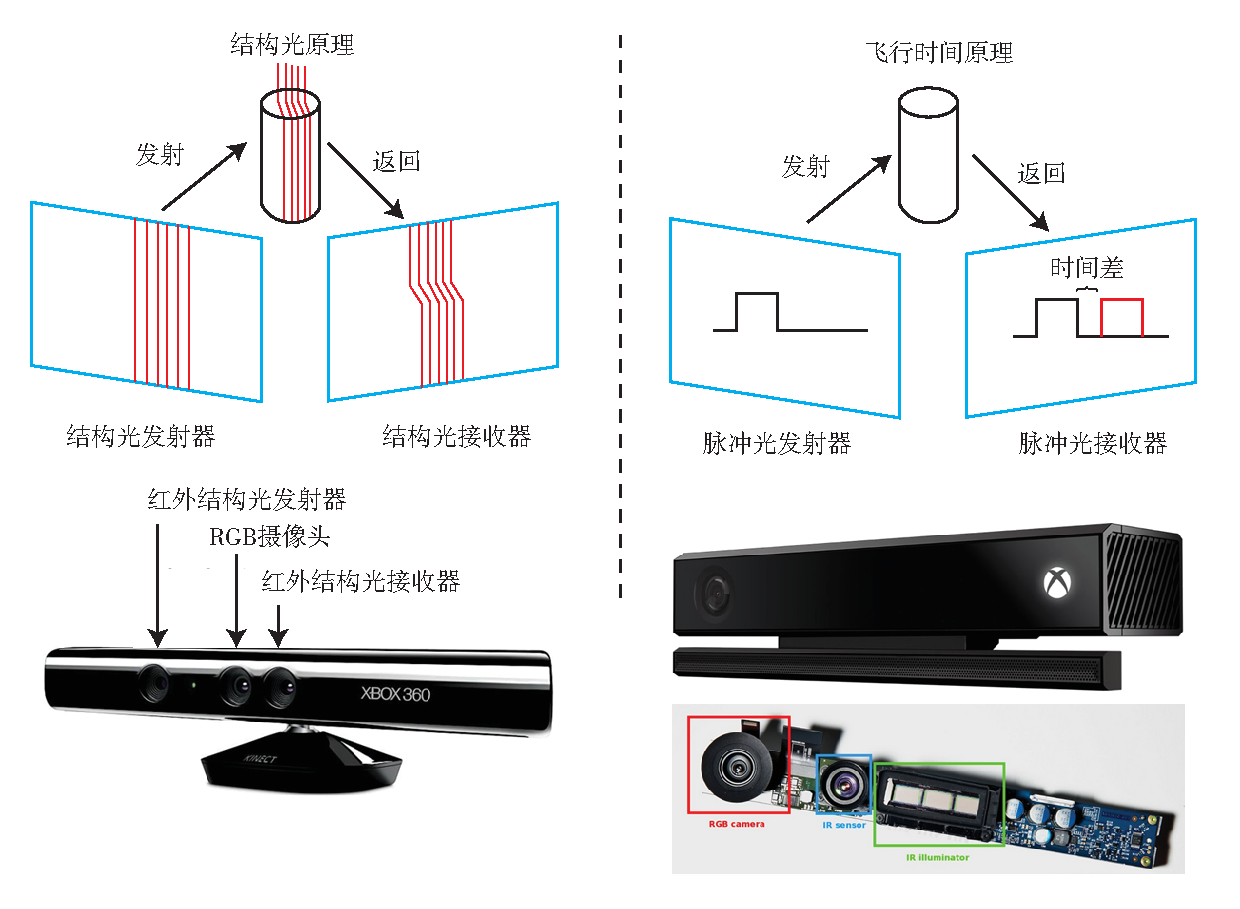
\includegraphics[width=1.0\textwidth]{cameraModel/rgbdCamera.pdf}
	\caption{RGB-D相机原理示意图。}
	\label{fig:RGBDCamera}
\end{figure}

无论是哪种类型,RGB-D相机都需要向探测目标发射一束光线(通常是红外光)。在结构光原理中,相机根据返回的结构光图案,计算物体与自身之间的距离。而在ToF原理中,相机向目标发射脉冲光,然后根据发送到返回之间的光束飞行时间,确定物体与自身之间的距离。ToF原理和激光传感器十分相似,只不过激光是通过逐点扫描来获取距离,而ToF相机则可以获得整个图像的像素深度,这也正是RGB-D相机的特点。所以,如果你把一个RGB-D相机拆开,通常会发现除了普通的摄像头之外,至少会有一个发射器和一个接收器。

在测量深度之后,RGB-D相机通常按照生产时的各相机摆放位置,自己完成深度与彩色图像素之间的配对,输出一一对应的彩色图和深度图。我们可以在同一个图像位置,读取到色彩信息和距离信息,计算像素的3D相机坐标,生成点云(Point Cloud)。对RGB-D数据,既可以在图像层面进行处理,亦可在点云层面处理。本讲的第二个实验将演示RGB-D相机的点云构建过程。

RGB-D相机能够实时地测量每个像素点的距离。但是,由于这种发射−接收的测量方式,其使用范围比较受限。用红外光进行深度值测量的RGB-D相机,容易受到日光或其他传感器发射的红外光干扰,因此不能在室外使用。在没有调制的情况下,同时使用多个RGB-D相机时也会相互干扰。对于透射材质的物体,因为接收不到反射光,所以无法测量这些点的位置。此外,RGB-D相机在成本、功耗方面,都有一些劣势。

% TODO 鱼眼相机模型

\section{图像}
相机加上镜头,把三维世界中的信息转换成了一张由像素组成的照片,随后存储在计算机中,作为后续处理的数据来源。在数学中,图像可以用一个矩阵来描述;而在计算机中,它们占据一段连续的磁盘或内存空间,可以用二维数组来表示。这样一来,程序就不必区别它们处理的是一个数值矩阵,还是有实际意义的图像了。

本节,我们将介绍计算机图像处理的一些基本操作。特别地,通过OpenCV中图像数据的处理,理解计算机中处理图像的常见步骤,为后续章节打下基础。我们从最简单的图像——灰度图说起。在一张灰度图中,每个像素位置$(x,y)$对应一个灰度值$I$,所以,一张宽度为$w$、高度为$h$的图像,数学上可以记为一个函数:
\[
{I} (x,y): \mathbb{R}^2 \mapsto \mathbb{R}.
\]
其中$(x,y)$是像素的坐标。然而,计算机并不能表达实数空间,所以我们需要对下标和图像读数在某个范围内进行量化。例如$x,y$通常是0开始的整数。在常见的灰度图中,用0\textasciitilde255的整数(即一个unsigned char,1个字节)来表达图像的灰度读数。那么,一张宽度为640像素、高度为480像素分辨率的灰度图就可以表示为:

\begin{lstlisting}[language=C++, caption=二维数组表达图像]
unsigned char image[480][640];
\end{lstlisting}

为什么这里的二维数组是480$\times$640呢?因为在程序中,图像以二维数组形式存储。它的第一个下标是指数组的行,而第二个下标则是列。在图像中,数组的行数对应图像的高度,而列数对应图像的宽度。

下面考察这幅图像的内容。图像自然是由像素组成的。当访问某一个像素时,需要指明它所处的坐标,如\autoref{fig:imagesInComputer}~所示。该图左边显示了传统像素坐标系的定义方式。像素坐标系原点位于图像的左上角,$X$轴向右,$Y$轴向下(也就是前面所说的$u,v$坐标)。如果它还有第三个轴——$Z$轴,那么根据右手法则,$Z$轴应该是向前的。这种定义方式是与相机坐标系一致的。我们平时说的图像的宽度或列数,对应着$X$轴;而图像的行数或高度,则对应着它的$Y$轴。

\begin{figure}[!t]
	\centering
	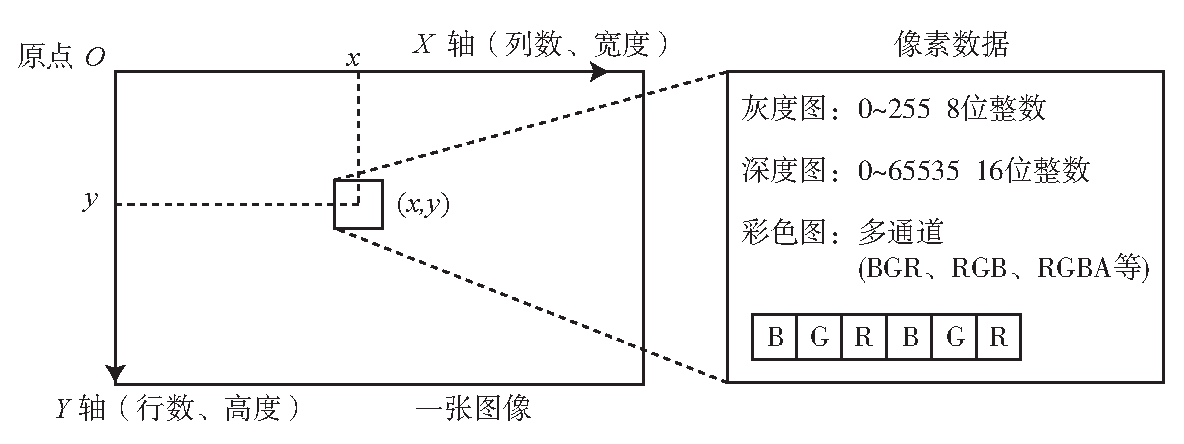
\includegraphics[width=0.84\textwidth]{cameraModel/image.pdf}
	\caption{图像坐标示意图。}
	\label{fig:imagesInComputer}
\end{figure}
	
根据这种定义方式,如果我们讨论一个位于$x,y$处的像素,那么它在程序中的访问方式应该是:
\begin{lstlisting}[language=C++, caption=访问图像像素]
unsigned char pixel = image[y][x];
\end{lstlisting}

它对应着灰度值$I(x,y)$的读数。请注意这里的$x$和$y$的顺序。虽然我们不厌其烦地讨论坐标系的问题,但是像这种下标顺序的错误,仍会是新手在调试过程中经常碰到的,且具有一定隐蔽性的错误之一。如果你在写程序时不慎调换了$x,y$的坐标,编译器无法提供任何信息,而你所能看到的只是程序运行中的一个越界错误而已。

一个像素的灰度可以用8位整数记录,也就是一个0\textasciitilde255的值。当我们要记录的信息更多时,一个字节恐怕就不够了。例如,在RGB-D相机的深度图中,记录了各个像素与相机之间的距离。这个距离通常是以毫米为单位,而RGB-D相机的量程通常在十几米左右,超过了255。这时,人们会采用16位整数(C++中的unsigned short)来记录深度图的信息,也就是位于0\textasciitilde65535的值。换算成米的话,最大可以表示65米,足够RGB-D相机使用了。

彩色图像的表示则需要通道(channel)的概念。在计算机中,我们用红色、绿色和蓝色这三种颜色的组合来表达任意一种色彩。于是对于每一个像素,就要记录其R、G、B三个数值,每一个数值就称为一个通道。例如,最常见的彩色图像有三个通道,每个通道都由8位整数表示。在这种规定下,一个像素占据24位空间。

通道的数量、顺序都是可以自由定义的。在OpenCV的彩色图像中,通道的默认顺序是B、G、R。也就是说,当我们得到一个24位的像素时,前8位表示蓝色数值,中间8位为绿色数值,最后8位为红色数值。同理,亦可使用R、G、B的顺序表示一个彩色图。如果还想表达图像的透明度,就使用R、G、B、A四个通道。

\section{实践:计算机中的图像}
\subsection{OpenCV的基础使用方法}
下面通过一个演示程序来理解,在OpenCV中图像是如何存取,而我们又是如何访问其中的像素的。

\subsubsection{安装OpenCV}
OpenCV\footnote{官方主页:\url{http://opencv.org}。}提供了大量的开源图像算法,是计算机视觉中使用极广的图像处理算法库。本书也使用OpenCV做基本的图像处理。在使用之前,建议读者从源代码安装它。在Ubuntu下,有\textbf{从源代码安装}和\textbf{只安装库文件}两种方式可以选择:

\begin{enumerate}
	\item 从源代码安装,是指从OpenCV网站下载所有的OpenCV源代码,并在机器上编译安装,以便使用。好处是可以选择的版本比较丰富,而且能看到源代码,不过需要花费一些编译时间。
	\item 只安装库文件,是指通过Ubuntu来安装由Ubuntu社区人员已经编译好的库文件,这样就无须重新编译一遍。
\end{enumerate}

由于我们使用较新版本的OpenCV,所以必须从源代码来安装它。一来,可以调整一些编译选项,匹配编程环境(例如,需不需要GPU加速等);再者,源代码安装可以使用一些额外的功能。OpenCV目前维护了两个主要版本,分为OpenCV 2.4系列和OpenCV 3系列。本书使用OpenCV \textbf{3}系列。

由于OpenCV工程比较大,就不放在本书的3rdparty下了。请读者从~\url{http://opencv.org/downloads.html}~下载,选择OpenCV for Linux版本即可。你会获得一个像opencv-3.1.0.zip这样的压缩包。将它解压到任意目录下,我们发现OpenCV亦是一个cmake工程。

在编译之前,先来安装OpenCV的依赖项:
\begin{lstlisting}[language=sh,caption=终端输入:]
sudo apt-get install build-essential libgtk2.0-dev libvtk5-dev libjpeg-dev libtiff4-dev libjasper-dev libopenexr-dev libtbb-dev
\end{lstlisting}

事实上,OpenCV的依赖项很多,缺少某些编译项会影响它的部分功能(不过我们也不会用到所有功能)。OpenCV会在cmake阶段检查依赖项是否会安装,并调整自己的功能。如果你的电脑上有GPU并且安装了相关依赖项,OpenCV也会把GPU加速打开。不过对于本书,上面那些依赖项就足够了。

随后的编译安装和普通的cmake工程一样,请在make之后,调用sudo make install将OpenCV安装到你的机器上(而不是仅仅编译它)。视机器配置,这个编译过程大概需要二十分钟到一个小时不等。如果你的CPU比较强,可以使用“make -j4”这样的命令,调用多个线程进行编译(-j后面的参数就是使用的线程数量)。安装后,OpenCV默认存储在/usr/local目录下。你可以去寻找OpenCV头文件与库文件的安装位置,看看它们都在哪里。另外,如果之前已经安装了OpenCV 2系列,那么建议你把OpenCV 3安装到别的地方(想想这应该如何操作)。

\subsubsection{操作OpenCV图像}
接下来通过一个例程熟悉一下OpenCV对图像的操作。
\begin{lstlisting}[language=C++,caption=slambook/ch5/imageBasics/imageBasics.cpp]
#include <iostream>
#include <chrono>

using namespace std;

#include <opencv2/core/core.hpp>
#include <opencv2/highgui/highgui.hpp>

int main(int argc, char **argv) {
	// 读取argv[1]指定的图像
	cv::Mat image;
	image = cv::imread(argv[1]); //cv::imread函数读取指定路径下的图像
	
	// 判断图像文件是否正确读取
	if (image.data == nullptr) { //数据不存在,可能是文件不存在
		cerr << "文件" << argv[1] << "不存在." << endl;
		return 0;
	}
	
	// 文件顺利读取, 首先输出一些基本信息
	cout << "图像宽为" << image.cols << ",高为" << image.rows 
	     << ",通道数为" << image.channels() << endl;
	cv::imshow("image", image);      // 用cv::imshow显示图像
	cv::waitKey(0);                  // 暂停程序,等待一个按键输入
	
	// 判断image的类型
	if (image.type() != CV_8UC1 && image.type() != CV_8UC3) {
		// 图像类型不符合要求
		cout << "请输入一张彩色图或灰度图." << endl;
		return 0;
	}
	
	// 遍历图像, 请注意以下遍历方式亦可使用于随机像素访问
	// 使用 std::chrono 来给算法计时
	chrono::steady_clock::time_point t1 = chrono::steady_clock::now();
	for (size_t y = 0; y < image.rows; y++) {
		// 用cv::Mat::ptr获得图像的行指针
		unsigned char *row_ptr = image.ptr<unsigned char>(y);  // row_ptr是第y行的头指针
		for (size_t x = 0; x < image.cols; x++) {
			// 访问位于 x,y 处的像素
			unsigned char *data_ptr = &row_ptr[x * image.channels()]; // data_ptr 指向待访问的像素数据
			// 输出该像素的每个通道,如果是灰度图就只有一个通道
			for (int c = 0; c != image.channels(); c++) {
				unsigned char data = data_ptr[c]; // data为I(x,y)第c个通道的值
			}
		}
	}
	chrono::steady_clock::time_point t2 = chrono::steady_clock::now();
	chrono::duration<double> time_used = chrono::duration_cast < chrono::duration < double >> (t2 - t1);
	cout << "遍历图像用时:" << time_used.count() << " 秒。" << endl;
	
	// 关于 cv::Mat 的拷贝
	// 直接赋值并不会拷贝数据
	cv::Mat image_another = image;
	// 修改 image_another 会导致 image 发生变化
	image_another(cv::Rect(0, 0, 100, 100)).setTo(0); // 将左上角100*100的块置零
	cv::imshow("image", image);
	cv::waitKey(0);
	
	// 使用clone函数来拷贝数据
	cv::Mat image_clone = image.clone();
	image_clone(cv::Rect(0, 0, 100, 100)).setTo(255);
	cv::imshow("image", image);
	cv::imshow("image_clone", image_clone);
	cv::waitKey(0);
	
	// 对于图像还有很多基本的操作,如剪切,旋转,缩放等,限于篇幅就不一一介绍了,请参看OpenCV官方文档查询每个函数的调用方法.
	cv::destroyAllWindows();
	return 0;
}
\end{lstlisting}
	
在该例程中,我们演示了如下几个操作:图像读取、显示、像素遍历、复制、赋值等。大部分的注解已写在代码里面。编译该程序时,你需要在CMakeLists.txt中添加OpenCV的头文件,然后把程序链接到库文件上。同时,由于使用了C++ 11标准(如nullptr和chrono),还需要设置一下编译器:

\begin{lstlisting}[language=Python,caption=slambook/ch5/imageBasics/CMakeLists.txt]
# 添加 C++ 11 标准支持
set( CMAKE_CXX_FLAGS "-std=c++11" )

# 寻找 OpenCV 库
find_package( OpenCV REQUIRED )
# 添加头文件
include_directories( ${OpenCV_INCLUDE_DIRS} )

add_executable( imageBasics imageBasics.cpp )
# 链接 OpenCV 库
target_link_libraries( imageBasics ${OpenCV_LIBS} )
\end{lstlisting}

关于代码,我们给出几点说明:
\begin{enumerate}
	\item 程序从argv[1],也就是命令行的第一个参数中读取图像位置。我们为读者准备了一张图像(ubuntu.png,一张Ubuntu的壁纸,希望你喜欢)供测试使用。因此,编译之后,使用如下命令调用此程序:
\begin{lstlisting}[language=sh,caption=终端输入:]
build/imageBasics ubuntu.png
\end{lstlisting}
	如果在IDE中调用此程序,请务必确保把参数同时给它。这可以在启动项中配置。
	\item 程序的10\textasciitilde18行,使用cv::imread函数读取图像,并把图像和基本信息显示\mbox{出来。}
	\item 在35\textasciitilde47行,遍历了图像中的所有像素,并计算了整个循环所用的时间。请注意像素的遍历方式并不是唯一的,而且例程给出的方式也不是最高效的。OpenCV提供了迭代器,你可以通过迭代器遍历图像的像素。或者,cv::Mat::data提供了指向图像数据开头的指针,你可以直接通过该指针自行计算偏移量,然后得到像素的实际内存位置。例程所用的方式是为了便于读者理解图像的结构。

	在笔者的机器上(虚拟机),遍历这张图像用时大约12.74ms。你可以对比一下自己机器上的速度。不过,我们使用的是cmake默认的debug模式,如果使用release模式会快很多。

	\item OpenCV提供了许多对图像进行操作的函数,我们在此不一一列举,否则本书就会变成OpenCV操作手册了。例程给出了较为常见的读取、显示操作,以及复制图像中可能陷入的深拷贝误区。在编程过程中,读者还会碰到图像的旋转、插值等操作,这时你应该自行查阅函数对应的文档,以了解它们的原理与使用方式。
\end{enumerate}

应该指出,OpenCV并不是唯一的图像库,它只是许多图像库里使用范围较广泛的一个。不过,多数图像库对图像的表达是大同小异的。我们希望读者了解了OpenCV对图像的表示后,能够理解其他库中图像的表达,从而在需要数据格式时能够自己处理。另外,由于cv::Mat亦是矩阵类,除了表示图像之外,我们也可以用它来存储位姿等矩阵数据。一般认为,Eigen对于固定大小的矩阵使用起来效率更高一些。

\subsection{图像去畸变}
在理论部分我们介绍了径向和切向畸变,下面来演示一个去畸变过程。OpenCV提供了去畸变函数cv::Undistort(),但本例我们从公式出发来计算一下畸变前后的图像坐标。
\begin{lstlisting}[language=C++,caption=slambook/ch5/imageBasics/undistortImage.cpp]
#include <opencv2/opencv.hpp>
#include <string>
using namespace std;
string image_file = "./distorted.png";   // 请确保路径正确

int main(int argc, char **argv) {
	// 本程序实现去畸变部分的代码。尽管我们可以调用OpenCV的去畸变,但自己实现一遍有助于理解。
	// 畸变参数
	double k1 = -0.28340811, k2 = 0.07395907, p1 = 0.00019359, p2 = 1.76187114e-05;
	// 内参
	double fx = 458.654, fy = 457.296, cx = 367.215, cy = 248.375;
	
	cv::Mat image = cv::imread(image_file, 0);   // 图像是灰度图,CV_8UC1
	int rows = image.rows, cols = image.cols;
	cv::Mat image_undistort = cv::Mat(rows, cols, CV_8UC1);   // 去畸变以后的图
	
	// 计算去畸变后图像的内容
	for (int v = 0; v < rows; v++) {
		for (int u = 0; u < cols; u++) {
			// 按照公式,计算点(u,v)对应到畸变图像中的坐标(u_distorted, v_distorted)
			double x = (u - cx) / fx, y = (v - cy) / fy;
			double r = sqrt(x * x + y * y);
			double x_distorted = x * (1 + k1 * r * r + k2 * r * r * r * r) + 2 * p1 * x * y + p2 * (r * r + 2 * x * x);
			double y_distorted = y * (1 + k1 * r * r + k2 * r * r * r * r) + p1 * (r * r + 2 * y * y) + 2 * p2 * x * y;
			double u_distorted = fx * x_distorted + cx;
			double v_distorted = fy * y_distorted + cy;
			
			// 赋值 (最近邻插值)
			if (u_distorted >= 0 && v_distorted >= 0 && u_distorted < cols && v_distorted < rows) {
				image_undistort.at<uchar>(v, u) = image.at<uchar>((int) v_distorted, (int) u_distorted);
			} else {
				image_undistort.at<uchar>(v, u) = 0;
			}
		}
	}
	
	// 画图去畸变后图像
	cv::imshow("distorted", image);
	cv::imshow("undistorted", image_undistort);
	cv::waitKey();
	return 0;
}
\end{lstlisting}

\section{实践:3D视觉}
\subsection{双目视觉}
我们已经介绍了双目视觉的成像原理。现在我们从双目的左右图像出发,计算图像对应的视差图,然后再计算各像素在相机坐标系下的坐标,它们将构成\textbf{点云}。在第五讲代码目录的stereo文件夹中,我们准备了左右目的图像,如\autoref{fig:stereoExample}所示。下面的代码演示了计算视差图和点云部分:
\begin{lstlisting}[language=C++,caption=slambook/ch5/stereoVision/stereoVision.cpp(部分)]
int main(int argc, char **argv) {
    // 内参
    double fx = 718.856, fy = 718.856, cx = 607.1928, cy = 185.2157;
    // 基线
    double b = 0.573;
    
    // 读取图像
    cv::Mat left = cv::imread(left_file, 0);
    cv::Mat right = cv::imread(right_file, 0);
    cv::Ptr<cv::StereoSGBM> sgbm = cv::StereoSGBM::create(
        0, 96, 9, 8 * 9 * 9, 32 * 9 * 9, 1, 63, 10, 100, 32);    // 神奇的参数
    cv::Mat disparity_sgbm, disparity;
    sgbm->compute(left, right, disparity_sgbm);
    disparity_sgbm.convertTo(disparity, CV_32F, 1.0 / 16.0f);
    
    // 生成点云
    vector<Vector4d, Eigen::aligned_allocator<Vector4d>> pointcloud;
    
    // 如果你的机器慢,请把后面的v++和u++改成v+=2, u+=2
    for (int v = 0; v < left.rows; v++)
        for (int u = 0; u < left.cols; u++) {
            if (disparity.at<float>(v, u) <= 10.0 || disparity.at<float>(v, u) >= 96.0) continue;
            
            Vector4d point(0, 0, 0, left.at<uchar>(v, u) / 255.0); // 前三维为xyz,第四维为颜色
            
            // 根据双目模型计算 point 的位置
            double x = (u - cx) / fx;
            double y = (v - cy) / fy;
            double depth = fx * b / (disparity.at<float>(v, u));
            point[0] = x * depth;
            point[1] = y * depth;
            point[2] = depth;
            
            pointcloud.push_back(point);
    }
    
    cv::imshow("disparity", disparity / 96.0);
    cv::waitKey(0);
    // 画出点云
    showPointCloud(pointcloud);
    return 0;
}
\end{lstlisting}

这个例子中我们调用了OpenCV实现的SGBM(Semi-global Batch Matching)\textsuperscript{\cite{Hirschmuller2008}}算法计算左右图像的视差,然后通过双目相机的几何模型把它变换到相机的3D空间中。SGBM使用了来自网络的经典参数配置,我们主要调整了最大和最小视差。视差数据结合相机的内参、基线,即能确定各点在三维空间中的位置。为了节省版面,我们省略了显示点云相关的代码。

\begin{figure}[!t]
    \centering
    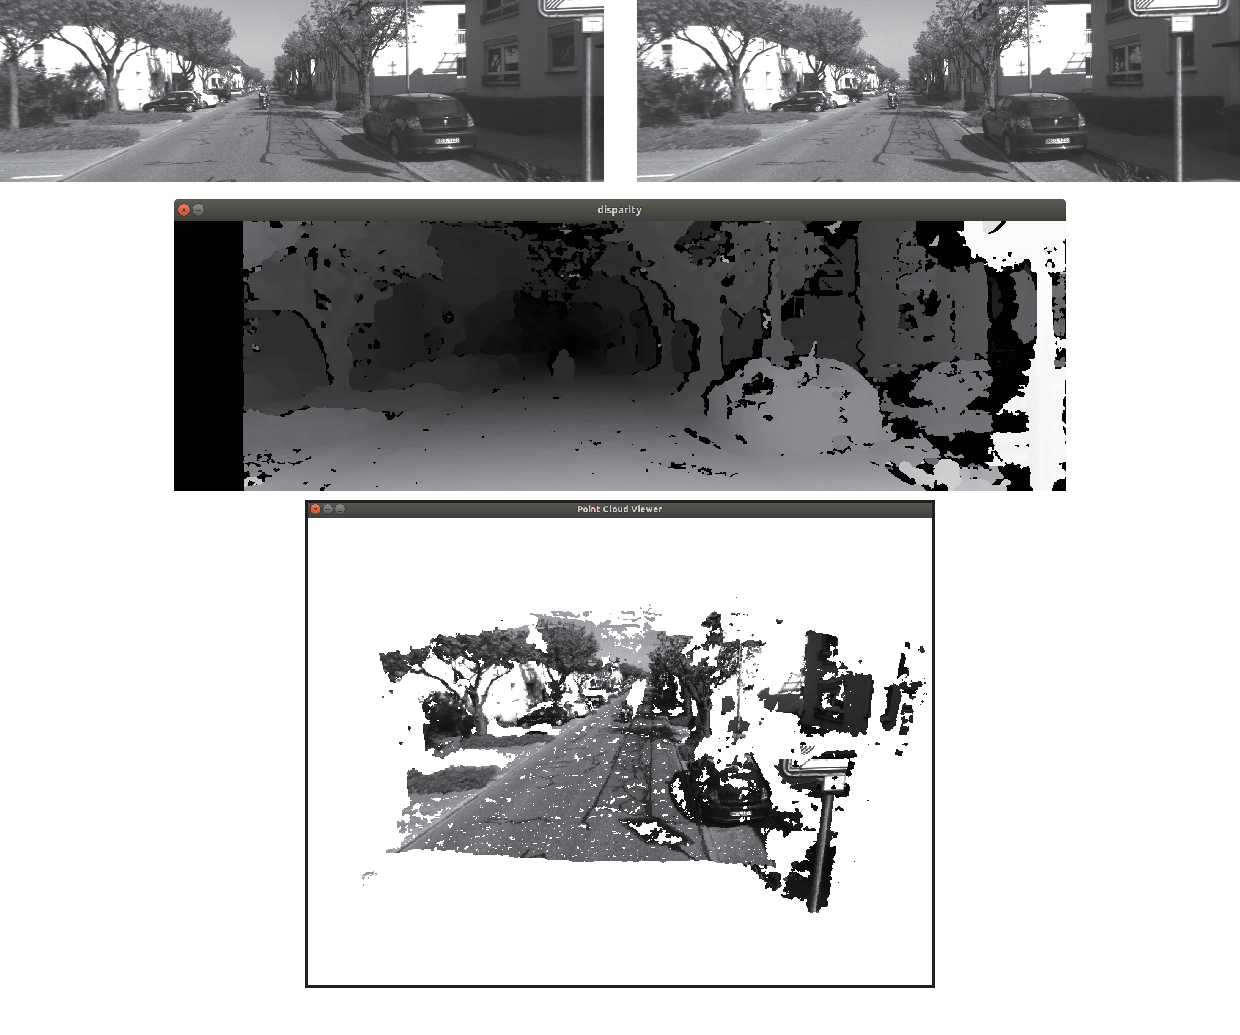
\includegraphics[width=0.9\textwidth]{cameraModel/stereoExample.pdf}
    \caption{双目视觉的例子,左上:左眼图像,右上:右眼图像,中间:SGBM的视差图,下方:点云图。注意左侧相机看到了一部分右侧相机没有看到的内容,所以对应的视差是空的。}
    \label{fig:stereoExample}
\end{figure}

本书不准备展开介绍双目相机的视差计算算法,感兴趣的读者可以阅读相关的参考文献\textsuperscript{\cite{Scharstein2002, Seitz2006}}。除了OpenCV实现的双目算法以外,还有许多其他的库专注于实现高效的视差计算。它是一个复杂又实用的课题。

\subsection{RGB-D视觉}
\label{sec:join-point-cloud}
最后,我们演示一个RGB-D视觉的例子。RGB-D相机的方便之处在于能通过物理方法获得像素深度信息。如果已知相机的内外参,我们可以计算任何一个像素在世界坐标系下的位置,从而建立一张点云地图。现在我们就来演示一下。

我们准备了5对图像,位于slambook/ch5/rgbd文件夹中。在color/下有1.png到5.png共5张RGB图,而在depth/下有5张对应的深度图。同时,pose.txt文件给出了5张图像的相机外参位姿(以$\bm{T}_\mathrm{wc}$形式)。位姿记录的形式和之前一样,为平移向量加旋转四元数:
\[
[x,y,z,q_x,q_y,q_z, q_w],
\]
其中$q_w$是四元数的实部。例如,第一对图的外参为:
\[
[-0.228993, 0.00645704, 0.0287837, -0.0004327, -0.113131, -0.0326832, 0.993042].
\]

下面我们写一段程序,完成两件事:(1). 根据内参计算一对RGB-D图像对应的点云;(2). 根据各张图的相机位姿(也就是外参),把点云加起来,组成地图。

\begin{lstlisting}[language=C++,caption=slambook/ch5/rgbd/jointMap.cpp(部分)]
int main(int argc, char **argv) {
    vector<cv::Mat> colorImgs, depthImgs;    // 彩色图和深度图
    TrajectoryType poses;         // 相机位姿
    
    ifstream fin("./pose.txt");
    if (!fin) {
        cerr << "请在有pose.txt的目录下运行此程序" << endl;
        return 1;
    }
    
    for (int i = 0; i < 5; i++) {
        boost::format fmt("./%s/%d.%s"); //图像文件格式
        colorImgs.push_back(cv::imread((fmt % "color" % (i + 1) % "png").str()));
        depthImgs.push_back(cv::imread((fmt % "depth" % (i + 1) % "pgm").str(), -1)); // 使用-1读取原始图像
        
        double data[7] = {0};
        for (auto &d:data) fin >> d;
        Sophus::SE3d pose(Eigen::Quaterniond(data[6], data[3], data[4], data[5]),
        Eigen::Vector3d(data[0], data[1], data[2]));
        poses.push_back(pose);
    }
    
    // 计算点云并拼接
    // 相机内参 
    double cx = 325.5;
    double cy = 253.5;
    double fx = 518.0;
    double fy = 519.0;
    double depthScale = 1000.0;
    vector<Vector6d, Eigen::aligned_allocator<Vector6d>> pointcloud;
    pointcloud.reserve(1000000);
    
    for (int i = 0; i < 5; i++) {
        cout << "转换图像中: " << i + 1 << endl;
        cv::Mat color = colorImgs[i];
        cv::Mat depth = depthImgs[i];
        Sophus::SE3d T = poses[i];
        for (int v = 0; v < color.rows; v++)
            for (int u = 0; u < color.cols; u++) {
                unsigned int d = depth.ptr<unsigned short>(v)[u]; // 深度值
                if (d == 0) continue; // 为0表示没有测量到
                Eigen::Vector3d point;
                point[2] = double(d) / depthScale;
                point[0] = (u - cx) * point[2] / fx;
                point[1] = (v - cy) * point[2] / fy;
                Eigen::Vector3d pointWorld = T * point;
                
                Vector6d p;
                p.head<3>() = pointWorld;
                p[5] = color.data[v * color.step + u * color.channels()];   // blue
                p[4] = color.data[v * color.step + u * color.channels() + 1]; // green
                p[3] = color.data[v * color.step + u * color.channels() + 2]; // red
                pointcloud.push_back(p);
            }
    }
    
    cout << "点云共有" << pointcloud.size() << "个点." << endl;
    showPointCloud(pointcloud);
    return 0;
}
\end{lstlisting}

运行程序后即可在Pangolin窗口中看到拼合的点云地图了(见\autoref{fig:pointcloudmapping})。你可以拖动鼠标查看。

\begin{figure}[!htp]
	\centering
	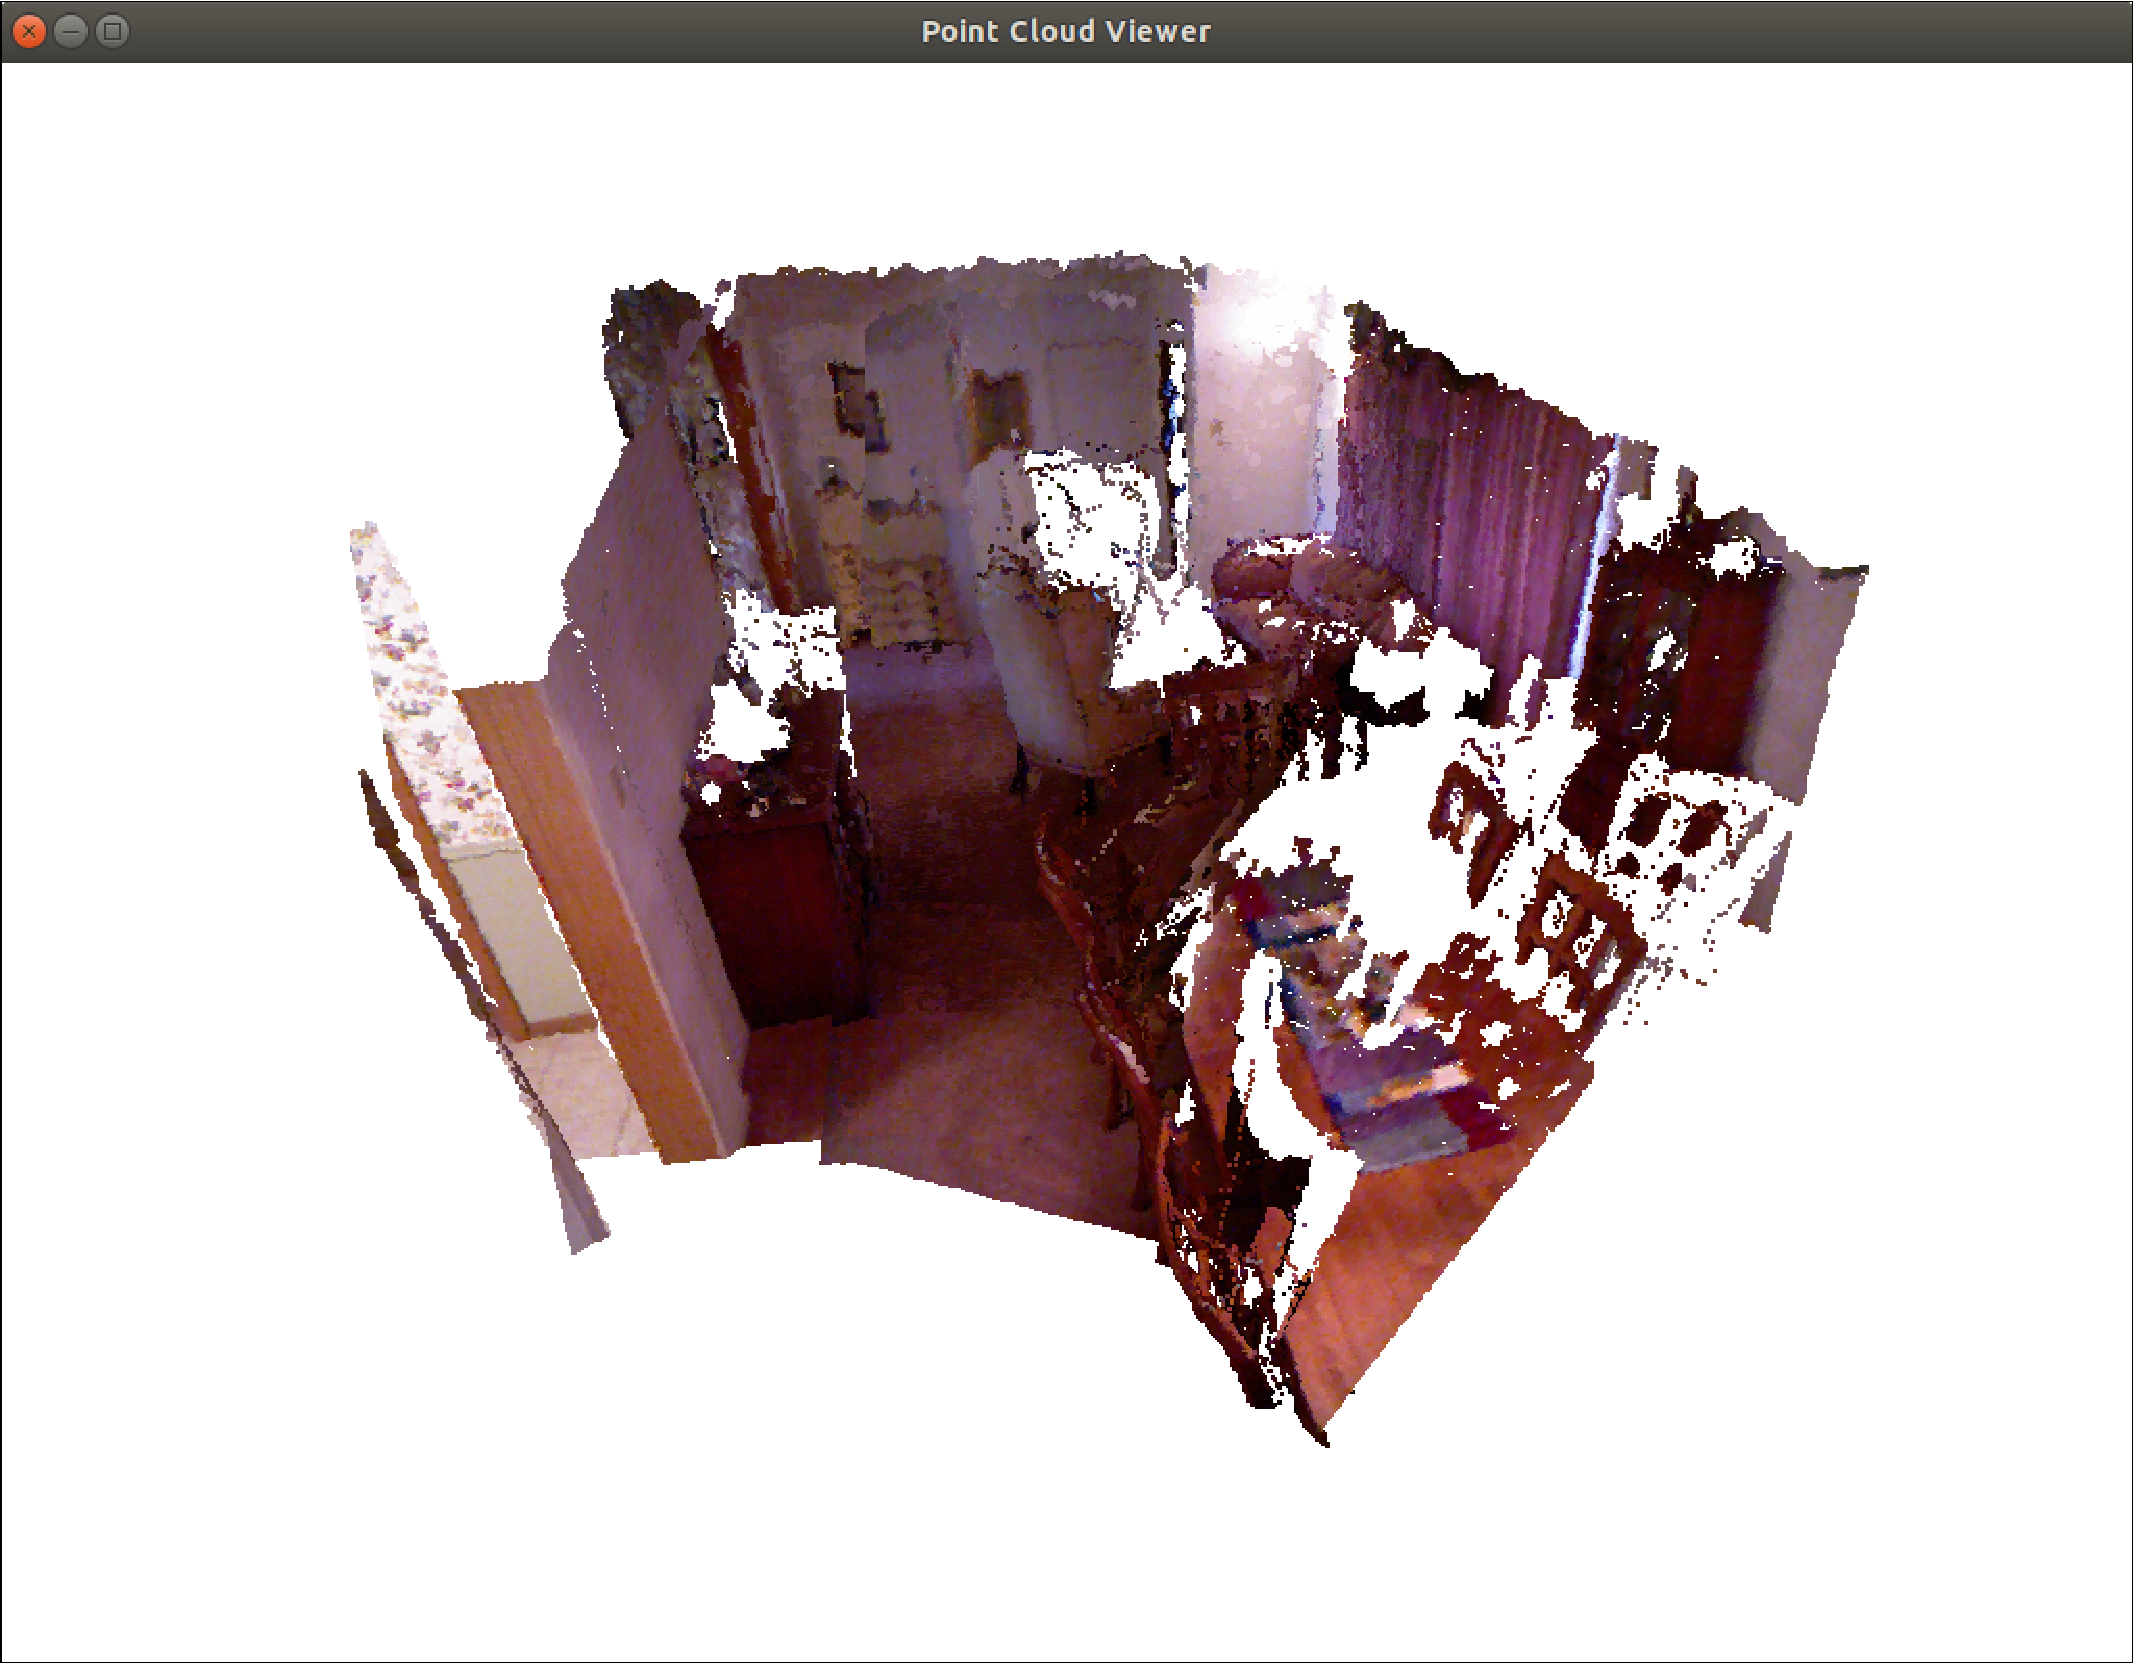
\includegraphics[width=1.0\textwidth]{cameraModel/pointcloud.pdf}
	\caption{查看拼合的点云地图。}
	\label{fig:pointcloudmapping}
\end{figure}

通过这些例子,我们演示了计算机视觉中一些常见的单目、双目和深度相机算法。希望读者通过这些简单的例子,实际地体会相机内外参、畸变参数的含义。

\section*{习题}
\begin{enumerate}
	\item[\optional] 寻找一部相机(你的手机或笔记本的摄像头即可),标定它的内参。你可能会用到标定板,或者自己打印一张标定用的棋盘格。
	\item 叙述相机内参的物理意义。如果一部相机的分辨率变为原来的两倍而其他地方不变,它的内参如何变化?
	\item 搜索特殊相机(鱼眼或全景相机)的标定方法。它们与普通的针孔模型有何\mbox{不同?}
	\item 调研全局快门相机(global shutter)和卷帘快门相机(rolling shutter)的异同。它们在SLAM中有何优缺点?
	\item RGB-D相机是如何标定的?以Kinect为例,需要标定哪些参数?(参照\url{https://github.com/code-iai/iai_kinect2}。)
	\item 除了示例程序演示的遍历图像的方式,你还能举出哪些遍历图像的方法?
	\item[\optional] 阅读OpenCV官方教程,学习它的基本用法。
\end{enumerate}
